

\section{Introduction}

Data Quality and Data Integration are two major problems which are becoming critical for health care providers everywhere. Research data is held on different systems, in different locations and the data itself is heterogeneous, collected without a common syntax or semantics. The successful application of metadata registries together with model driven engineering has been demonstrated to have a significant impact on these problems within two major healthcare projects within the UK's National Health Service(NHS).

The UK's National Institute for Health Research (NIHR \cite{NIHR}) has sponsored the Health Informatics Collaberative (NHIC) which is backing a cross-trust programme involving 5 key NHS hospital trusts in the UK in order to set up a flexible and responsive governance framework, whereby research outcomes can rapidly be exploited by the NHS community. The work is currently limited to 5 clinical areas, but is expected in time to be extended. One of the aims of the programme is to develop tools and services for research, so that researchers can clinicians can have access to a wider cross Biomedical Research Centre (BRC) dataset. The programme has been working on developing a federated metadata registry, based on the ISO standard for metadata registries ISO11179\cite{ISO11179}, for use as a basis for enabling interoperability primarily for research data from clinical trials but also with a view to integrating this capability with Electronic Patient Records (EPR) data within the trusts.

Genomics England (GEL \cite{GEL}) is a research company wholly owned by the UK's NHS, which has been created ......

\subsection{Background}
The idea of a data dictionary has been around since databases first become common instruments for storing and manipulating data. A data dictionary is  the idea of a metadata registry stems from a similar notion.
Metadata Registries are needed in organizations to ensure data consistency. Metadata Registries are capable of analysing, administering and classifying metadata and very often in practise they also function as repositories for metadata, storing the schema and blueprints for data types and structures. The ideas and concepts that are stored in data systems form the basis of executable software systems, however many of the details are peculiar to particular disciplines.  

In the past Data Dictionaries were used to store details of database record structure or application data structure on a local per application basis, a metadata registry provides a similar capability but on a system or organisation-wide basis. It also provides features that are commonly included in a \emph{thesaurus}, a \emph{Taxonomy}, and an \emph{Ontology} . These features include the ability to classify terms in relation to one another, record relationships such as synonyms, and classify hierarchical relationships.

Metadata Registries are normally found in Data Warehouses and Enterprise systems, where vast quantities of data need to be administered and managed. It is likely that metadata registries will become more common as it becomes more and more necessary to deal with the recent internet-driven data explosion, especially as much of this data is unstructured, and can only be processed by relatively inefficient techniques.

Metadata Registries contain the ability to examine both how a data element is represented as well as what it means, and it is this relationship that is embodied in the International Standard 11179, which I will examine in the next section. There are other standards which purport to be concerned with metadata registries namely ISO15000-3 and ISO15000-4, which relate to ebXML, however they are more concerned with storing and accessing metadata rather than classifying it and relating the semantic and representational aspects of that metadata.

\subsection{ISO11179}
ISO11179 is the international standard relating to metadata and in particular metadata registries, and although there are a few other related standards which I have examined in the course of specifying a metadata registry ISO11179 provides the most exhaustive description of a metadata registry. It is therefore a key reference in this specification. If we abstract the core ideas from the ISO11179 standard we have the notion of a \emph{data element concept}, \emph{a data element}, \emph{a value domain}, and a \emph{conceptual domain}. The standard has no notion of collections of data elements, but instead attaches two attributes: an \emph{object class} and a \emph{property} to each DEC, these attributes allow DEC's to be aggregated or classified, see figure\ref{fig:basicMDR}


\begin{figure}[here]
	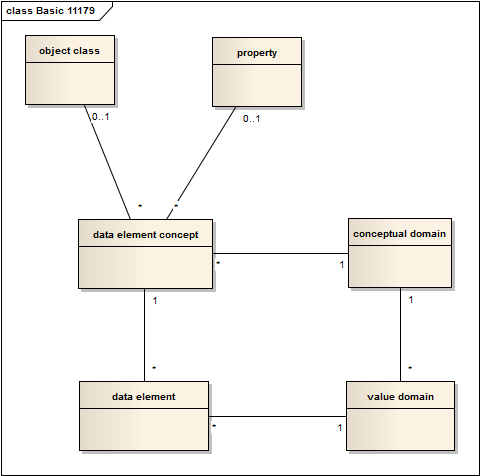
\includegraphics[width=0.5\textwidth,natwidth=610,natheight=642]{Basic11179}
	\caption{Core model for ISO11179 Metadata Registry} 
	\label{fig:basicMDR}
\end{figure}

ISO11179 is a very thorough standard for metadata registries, and is split into 6 sections.

\subsection{Related Work}
????

\subsection{Objectives}
This paper is an experience paper showing the results obtained from applying the principles of Model Driven Engineering to achieve solutions in the medical domain. In both cases the aims of the clinicians were similar, namely to integrate existing clinical trials data and to ensure that future artefacts, such as the forms used to capture datasets resulted in high data quality. The biggest frustration in fusing datasets is that it is a slow process requiring highly trained operators to ensure that datasets are correctly merged. 
The paper is split into 5 sections, this section introduces the problem and gives an overview of the work, the next section looks at the core language or model used, section 3 deals with the implementation details, section 4 details the experience gained, in essence the results achieved and section 5 concludes.
